\begin{figure}[h!]
	\centering
	
	
	
	\tikzset{every picture/.style={line width=0.75pt}} %set default line width to 0.75pt        
	
	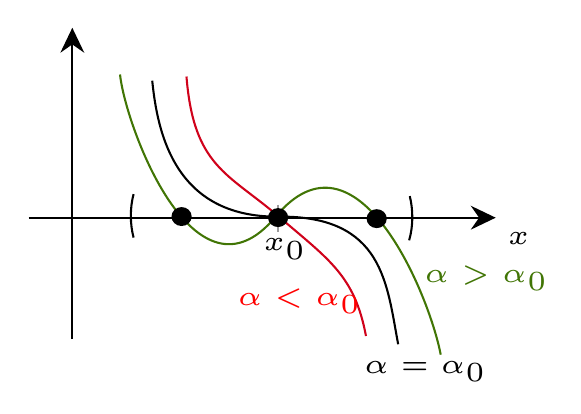
\begin{tikzpicture}[x=0.75pt,y=0.75pt,yscale=-1.5,xscale=1.5]
		%uncomment if require: \path (0,300); %set diagram left start at 0, and has height of 300
		
		%Straight Lines [id:da05892022845111411] 
		\draw    (217,100.67) -- (364,100.67) ;
		\draw [shift={(367,100.67)}, rotate = 180] [fill={rgb, 255:red, 0; green, 0; blue, 0 }  ][line width=0.08]  [draw opacity=0] (8.04,-3.86) -- (0,0) -- (8.04,3.86) -- (5.34,0) -- cycle    ;
		%Straight Lines [id:da806758973605693] 
		\draw    (231,139.67) -- (231,42.67) ;
		\draw [shift={(231,39.67)}, rotate = 90] [fill={rgb, 255:red, 0; green, 0; blue, 0 }  ][line width=0.08]  [draw opacity=0] (8.04,-3.86) -- (0,0) -- (8.04,3.86) -- (5.34,0) -- cycle    ;
		%Shape: Arc [id:dp6058068696964698] 
		\draw  [draw opacity=0] (250.68,107.06) .. controls (250.12,104.92) and (249.8,102.56) .. (249.8,100.07) .. controls (249.8,97.58) and (250.11,95.22) .. (250.68,93.1) -- (259.8,100.07) -- cycle ; \draw   (250.68,107.06) .. controls (250.12,104.92) and (249.8,102.56) .. (249.8,100.07) .. controls (249.8,97.58) and (250.11,95.22) .. (250.68,93.1) ;  
		%Shape: Arc [id:dp14042025356928334] 
		\draw  [draw opacity=0] (339.39,93.74) .. controls (339.91,95.81) and (340.2,98.08) .. (340.2,100.47) .. controls (340.2,103.14) and (339.84,105.68) .. (339.19,107.93) -- (330.2,100.47) -- cycle ; \draw   (339.39,93.74) .. controls (339.91,95.81) and (340.2,98.08) .. (340.2,100.47) .. controls (340.2,103.14) and (339.84,105.68) .. (339.19,107.93) ;  
		%Straight Lines [id:da25297557942373183] 
		\draw [color={rgb, 255:red, 155; green, 155; blue, 155 }  ,draw opacity=1 ]   (297.2,96.47) -- (297.2,105.27) ;
		%Curve Lines [id:da9485721249224925] 
		\draw [color={rgb, 255:red, 208; green, 2; blue, 27 }  ,draw opacity=1 ]   (267.67,55.33) .. controls (270,84.33) and (281,86.33) .. (297.33,100.33) .. controls (313.67,114.33) and (321.67,119.33) .. (325.33,138.67) ;
		%Curve Lines [id:da7115178345870963] 
		\draw [color={rgb, 255:red, 0; green, 0; blue, 0 }  ,draw opacity=1 ]   (256.67,56.67) .. controls (258.33,73) and (263.67,100.67) .. (297.33,100.33) .. controls (331,100) and (332,122) .. (335.67,141.33) ;
		%Curve Lines [id:da8498861454657496] 
		\draw [color={rgb, 255:red, 65; green, 117; blue, 5 }  ,draw opacity=1 ]   (246.33,54.67) .. controls (248,71) and (270.33,131.67) .. (296.33,100.33) .. controls (322.33,69) and (345.67,125.33) .. (349.33,144.67) ;
		%Shape: Path Data [id:dp508632932098046] 
		\draw  [fill={rgb, 255:red, 0; green, 0; blue, 0 }  ,fill opacity=1 ] (294.2,100.63) .. controls (294.2,99.14) and (295.5,97.93) .. (297.1,97.93) .. controls (298.7,97.93) and (300,99.14) .. (300,100.63) .. controls (300,102.12) and (298.7,103.33) .. (297.1,103.33) .. controls (295.5,103.33) and (294.2,102.12) .. (294.2,100.63) -- cycle ;
		%Shape: Path Data [id:dp4059785824642126] 
		\draw  [fill={rgb, 255:red, 0; green, 0; blue, 0 }  ,fill opacity=1 ] (263.2,100.3) .. controls (263.2,98.81) and (264.5,97.6) .. (266.1,97.6) .. controls (267.7,97.6) and (269,98.81) .. (269,100.3) .. controls (269,101.79) and (267.7,103) .. (266.1,103) .. controls (264.5,103) and (263.2,101.79) .. (263.2,100.3) -- cycle ;
		%Shape: Path Data [id:dp2560720790739939] 
		\draw  [fill={rgb, 255:red, 0; green, 0; blue, 0 }  ,fill opacity=1 ] (325.87,100.97) .. controls (325.87,99.48) and (327.17,98.27) .. (328.77,98.27) .. controls (330.37,98.27) and (331.67,99.48) .. (331.67,100.97) .. controls (331.67,102.46) and (330.37,103.67) .. (328.77,103.67) .. controls (327.17,103.67) and (325.87,102.46) .. (325.87,100.97) -- cycle ;
		
		% Text Node
		\draw (290.4,105.47) node [anchor=north west][inner sep=0.75pt]  [font=\tiny,xscale=2,yscale=2]  {$x_{0}$};
		% Text Node
		\draw (368.8,103.47) node [anchor=north west][inner sep=0.75pt]  [font=\tiny,xscale=2,yscale=2]  {$x$};
		% Text Node
		\draw (342,114.07) node [anchor=north west][inner sep=0.75pt]  [font=\tiny,color={rgb, 255:red, 65; green, 117; blue, 5 }  ,opacity=1 ,xscale=2,yscale=2]  {$\alpha  >\alpha _{0}$};
		% Text Node
		\draw (282,121.4) node [anchor=north west][inner sep=0.75pt]  [font=\tiny,color={rgb, 255:red, 255; green, 0; blue, 0 }  ,opacity=1 ,xscale=2,yscale=2]  {$\alpha < \alpha _{0}$};
		% Text Node
		\draw (322.67,144.73) node [anchor=north west][inner sep=0.75pt]  [font=\tiny,xscale=2,yscale=2]  {$\alpha =\alpha _{0}$};
		
		
	\end{tikzpicture}
\end{figure}